\chapter{Interactive Visual Odometry on the Web}%
\label{cha:interactive_vo_on_the_web}

\minitoc%
\clearpage

\section{RGB-D Visual Odometry Evaluation}%
\label{sec:rgbd-vo-evaluation}

As previously explained, our implementation
belongs to the family of direct visual odometry from RGB-D images.
In this section, we will detail how it has been evaluated against
comparable algorithms by introducing the available datasets,
presenting the different evaluation metrics,
and finally lay out the testing setup we provide with the evaluation results.

\subsection{Dataset Creation / Aqcuisition}%
\label{sub:dataset_creation}

Comparing different algorithms is a complex task for many reasons.
One of them being the ability to run those algorithms on the same set of data.
The existence of well built reference datasets is thus a crucial point,
and understanding their caracteristics is valuable to correctly compare and interpret
evaluation results.

\subsubsection{Overview of Avalaible Datasets}%
\label{ssub:datasets_overview}

We saw in Chapter~\ref{cha:the_image_annotation_problem} that the principal
difficulty for building annotation datasets is the required human annotation time.
For visual odometry, algorithms are strongly related to capture devices,
be it stereo, mono, RGB-D cameras, or cameras paired with other sensors
such as inertial measurement units (IMU), GPS or lidar.
As a consequence, datasets focus on different acquisition systems.
For every evaluated acquisition system, there must exist another measurement system,
more precise and reliable than the one being evaluated.
The main difference is thus that
the challenge is technological for visual odometry,
while it is mostly time consumption for image annotation.

The availability of datasets for visual odometry first came from the mobile robotics community,
mostly interested in SLAM from laser sensors (lidar).
The data is thus collected from sensors attached to a mobile robot or car navigating.
In the New College~\cite{smith2009new} and NCLT~\cite{carlevaris2016university} datasets,
the robotic platform is based on a Segway, the KITTI dataset~\cite{geiger2013vision}
recorded data from a sensors equiped car,
while the EuRoC MAV~\cite{burri2016euroc}
dataset is based on a MAV flying robot.
These platforms are depicted in Figure~\ref{fig:mobile-robot-slam}.
The ground truth was recorded with three different approaches for these datasets.
Visual odometry ground truth was an after thought for the New College dataset,
only available a year later on their website and not discussed in the paper.
It seems that it has been obtained from dead-reckoning, i.e.\ from wheel and IMU odometry,
provided by the Segway platform, and is thus not very reliable.
In the NCLT dataset, the mobile robot trajectory ground truth is computed from
a high precision realtime kinematic GPS (RTK GPS) and a graph slam based on lidar measurements.
The accuracy of the trajectory ranges from a centimeter to a decimeter approximately for a total
travelled distance of roughly 147 km.
The ground truth trajectory of the KITTI dataset was also obtained from high precision
GPS/IMU sensors and is thus also accurate at the decimeter scale.
The setup for the EuRoC MAV dataset is a bit different since the mobile vehicle
is flying in indoor environment and its trajectory is obtained from motion capture devices.
The total travelled distance is thus way shorter, less than a kilometer,
but the trajectories are accurate at approximately a millimeter.

\begin{figure}[ht]
	\centering
	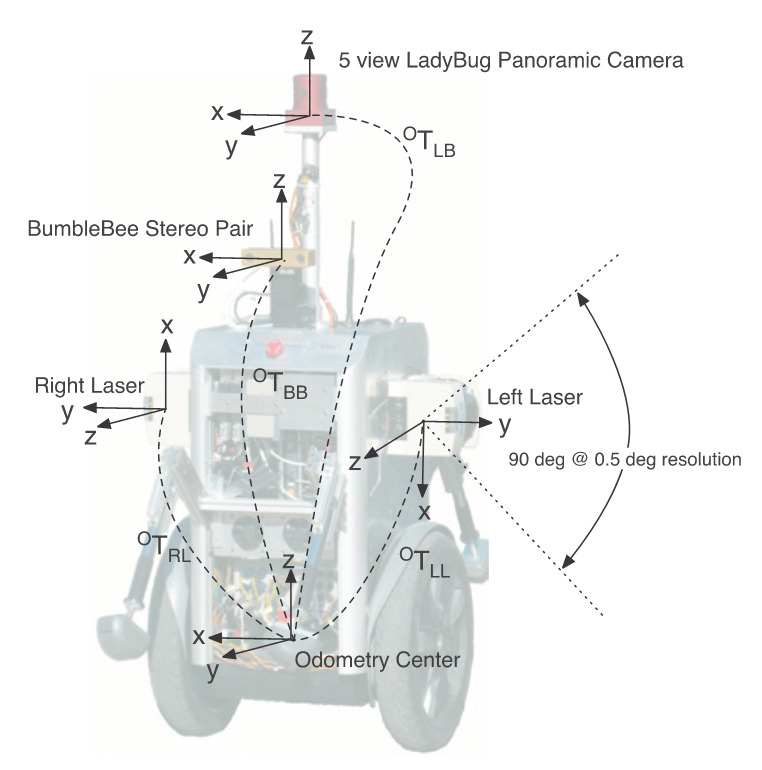
\includegraphics[height=0.3\linewidth]{assets/img/new-college.png}
	\hfill
	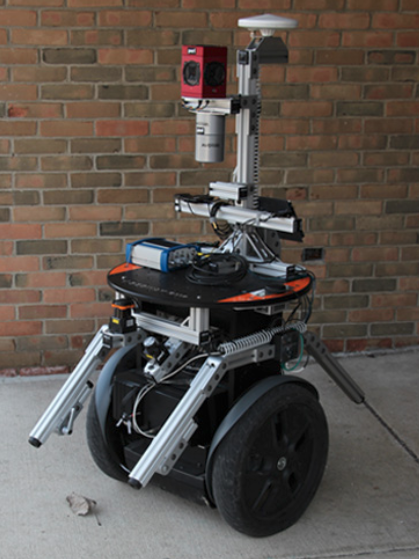
\includegraphics[height=0.3\linewidth]{assets/img/nclt.png}
	\hfill
	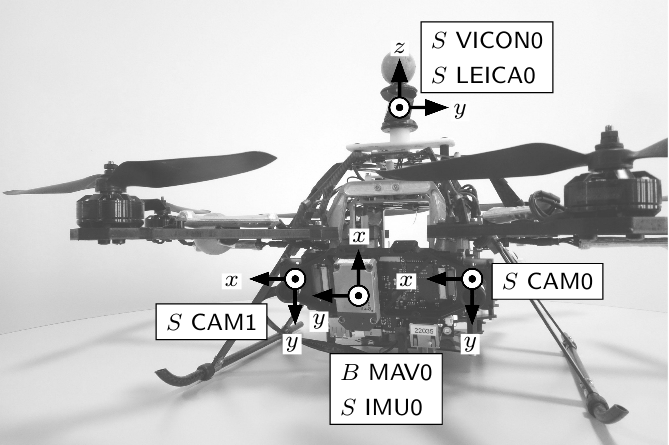
\includegraphics[height=0.3\linewidth]{assets/img/euroc-mav.png}
	\caption{Mobile robots used for SLAM datasets. From left to right,
	the Segway platform used in the New College dataset~\cite{smith2009new},
	the Segway platform used in the NCLT dataset~\cite{carlevaris2016university},
	the MAV used in the EuRoC MAV dataset~\cite{burri2016euroc}.}%
	\label{fig:mobile-robot-slam}
\end{figure}

A second wave of datasets has especially being targetting RGB-D cameras,
very popular after the launch of the Microsoft Kinect,
represented in bold in Table~\ref{tab:vo-datasets}.
While the TUM RGB-D~\cite{sturm2012benchmark} and Bonn RGB-D~\cite{palazzolo2019iros}
datasets are recorded with real RGB-D sensors,
the ICL-NUIM~\cite{handa2014benchmark} dataset was generated (ray-traced rendered)
from synthetic 3D models of indoor scenes.
We are going to explain in more details the specificities of the TUM RGB-D and
ICL-NUIM datasets since these are the two we used to evaluate our direct RGB-D
visual odometry algorithm.

Finally, with the popularity of inertial sensors coupled with cameras in
modern smartphones enabling new augmented reality functionalities,
a regain in interest have been visible for 6 degrees of freedom visual inertial odometry (VIO).
While the EuRoC MAV~\cite{burri2016euroc} and TUM VI~\cite{schubert2018tum} datasets
are using high quality sensors,
the ADVIO dataset~\cite{cortes2018advio} is actually using regular smartphones sensors,
showing the importance of datasets with less precise data to improve algorithms robustness.
We provide a brief summary of these datasets properties in Table~\ref{tab:vo-datasets}.
Note that this is not an exhaustive list of available datasets but an overview
of the main ones for visual odometry.

\begin{table}[ht]
\centering
\resizebox{\textwidth}{!}{%
\begin{tabular}{llll}
Dataset
	& Year
    & Available data
	& Ground truth \\
    \midrule
New College~\cite{smith2009new}
	& 2009
	& \makecell[l]{GPS, IMU, wheel odometry,\\lidar, omnidirectional, stereo}
	& Dead-reckoned \\
\textbf{TUM RGB-D~\cite{sturm2012benchmark}}
	& 2012
	& IMU, \textbf{RGB-D}
	& Motion capture \\
KITTI~\cite{geiger2013vision}
	& 2013
	& GPS, IMU, lidar, stereo
	& High precision GPS/IMU \\
\textbf{ICL-NUIM~\cite{handa2014benchmark}}
	& 2014
	& \textbf{RGB-D}, 3D surface
	& Synthetic \\
NCLT~\cite{carlevaris2016university}
	& 2016
	& \makecell[l]{GPS, IMU, wheel odometry,\\lidar, omnidirectional}
	& RTK GPS and lidar SLAM \\
EuRoC MAV~\cite{burri2016euroc}
	& 2016
	& Stereo camera
	& Motion capture \\
TUM Mono~\cite{engel2016photometrically}
	& 2016
	& Mono camera
	& Closed loop \\
TUM VI~\cite{schubert2018tum}
	& 2018
	& IMU, Mono camera
	& Motion capture and closed loop \\
ADVIO~\cite{cortes2018advio}
	& 2018
	& Smartphone IMU and video
	& IMU with position fixes \\
\textbf{Bonn RGB-D~\cite{palazzolo2019iros}}
	& 2019
	& IMU, \textbf{RGB-D}, lidar
	& Motion capture \\
\end{tabular}%
} % end of resizebox
\caption{Visual odometry datasets}%
\label{tab:vo-datasets}
\end{table}


\subsubsection{Motion Capture for RGB-D Visual Odometry}%
\label{ssub:motion_capture}

The TUM RGB-D dataset~\cite{sturm2012benchmark} was the first
complete and rigorously detailed dataset for RGB-D visual odometry.
It is composed of 80 sequences, 47 for training with ground truth,
and 33 for validation only evaluated online, without ground truth.
The training sequences are arranged in six groups,
\begin{itemize}
\setlength\itemsep{-0.5em}
	\item testing and debugging (4 sequences), simple translation or rotation movements,
	\item handheld movements (11 sequences),
	\item robot movements (4 sequences),
	\item structure and texture (8 sequences), with difficult structure or texture patterns,
	\item dynamic objects (9 sequences),
	\item and object reconstruction (11 sequences).
\end{itemize}
As we can see, the dataset provides both easy sequences and sequences with
more difficult situations such as dynamic movements or poor textures
in the field of view of the camera.
It is thus a good benchmark of the robustness of visual odometry algorithms.
These sequences have been acquired by three different Kinect devices,
named fr1 (for ``Freiburg 1''), fr2 and fr3.
All their intrinsic parameters are availabe in the dataset.
The required robustness of the tested algorithms are also increased by the fact that
the color camera of the Kinect sensor has a rolling shutter.
Taking into account the caracteristics of our implementation,
we do not expect our algorithm to perform very well under those circumstances.

The ground truth camera poses are obtained thanks to an external motion capture system
based on MotionAnalysis~\cite{MotionAnalysis} hardware and software.
This setup is composed of eight 300 Hz Raptor-E high definition cameras,
equiped with infrared lights to illuminate passive markers attached to the Kinect.
After a detailed intrinsic and extrinsic parameters calibration of the system,
the authors estimate the relative position errors to be lower than 1 mm and 0.5 degrees.

\subsubsection{Synthetic Dataset Creation}%
\label{ssub:synthetic_dataset}

Most of the available visual odometry datasets lack a dense 3D surface ground truth
to be able to evaluate both the camera trajectory and the structure reconstruction.
To this end, Handa et al.\ created the ICL-NUIM dataset~\cite{handa2014benchmark}.
Contrary to most other datasets, the video sequences provided here are completely
generated by computer graphics, using the open-source ray tracing algorithm
POV-Ray~\cite{povray}.
The dataset is split into two rooms, a living room and an office,
and two scenarios, one noiseless and one with simulated noise.
The full pipeline is also provided as open source,
if one wishes to customize parts of it.
The geometry and some renders of the living room are displayed in Figure~\ref{fig:icl-nuim}.

\begin{figure}[t]
	\centering
	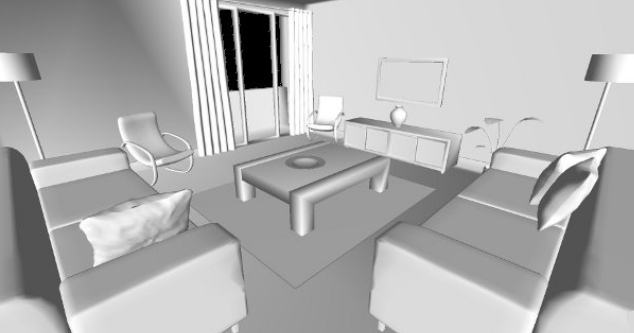
\includegraphics[height=0.3\linewidth]{assets/img/icl-nuim-geometry.png}
	\hfill
	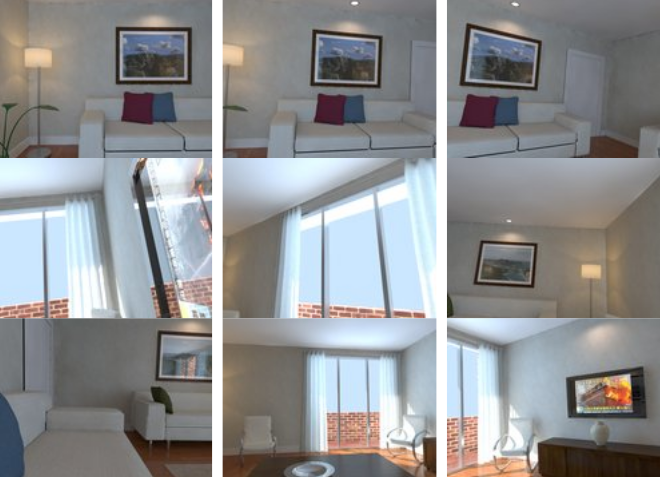
\includegraphics[height=0.3\linewidth]{assets/img/icl-nuim-povray.png}
	\caption{Geometry (left) and few rendered images (right)
	of the living room used for the ICL-NUIM dataset~\cite{handa2014benchmark}.}%
	\label{fig:icl-nuim}
\end{figure}

In order to test some visual odometry algorithms,
we are only going to use the eight noise-free sequences since realistic noisy sequences
are already evaluated with the TUM RGB-D dataset.
The trajectory ground truth generated by this ICL-NUIM dataset is thus error-free.
The color and depth images are also perfectly aligned,
timely synchronized and have no light exposure variations.
They still contain reflective surfaces and few other ligthing effects
not taken into account in our direct visual odometry modelization,
but the overall circumstances should be very favorable for our simple implementation.

\subsection{Evaluation Metrics}%
\label{sub:metrics}

There are basically two types of evaluation metrics,
those based on a ground truth, and those that are not.

\subsubsection{Metrics with Ground Truth, ATE and RPE}%
\label{ssub:metrics_gt}

The most straightforward method to evaluate visual odometry trajectories,
is to compare it with a reference trajectory, called ground truth.
This reference trajectory needs to be acquired by the system with more precision
than the one being evaluated for the measure to make sense.
In our case, the TUM RGB-D dataset uses a motion capture system with sub millimeter accuracy,
and the ICL-NUIM provides exact trajectory since it is a synthetic dataset.

The first evaluation metric commonly used is the absolute trajectory error (ATE).
Let's consider the trajectory as a discrete set of camera poses
\[
	G_{\Omega} = \Set{g_{\tau}}{\tau \in \Omega,\ g_{\tau} \in SE(3)}
\]
where $\Omega$ is the set of discrete time events when camera poses are available.
In theory, the ATE can be computed as
\[
	\text{ATE} = \sum_{\Omega} d(g_{\tau}, \widehat{g}_{\tau})
\]
where $d(g_{\tau}, \widehat{g}_{\tau})$ can be thought of
as a distance between the estimated transformation $g_{\tau}$
and the ground truth transformation $\widehat{g}_{\tau}$.
Usually, we can consider two types of errors, the translation error
\[
	\| \text{trans}(\inv{\widehat{g}_{\tau}} \cdot g_{\tau}) \|
\]
and the rotation error
\[
	\angle\ \text{rot}(\inv{\widehat{g}_{\tau}} \cdot g_{\tau})
\]
where $\angle$ is the amplitude ($\geq 0$) of the rotation angle.
Since the rotation errors will also impact translation errors later,
it is common to only use the translation error when computing the ATE.
The two most widely used ATE metrics are the RMSE and the median scores
\[
	\text{ATE}_{\text{rmse}} =
		\left( \mean{ \sum_{\Omega} \| \text{trans}(\inv{\widehat{g}_{\tau}} \cdot g_{\tau}) \|^2 }
		\right)^{1/2}
	\quad \text{and} \quad
	\text{ATE}_{\text{median}} =
		\text{median} \left( \| \text{trans}(\inv{\widehat{g}_{\tau}} \cdot g_{\tau}) \| \right).
\]
The median is a better indicator of the average algorithm precision,
while the RMSE better reflects the presence (or absence) of outliers,
i.e.\ the global robustness of the algorithm.

In practice, we should note that the ground truth and estimated trajectory
are not expressed in the same reference frame.
It is thus necessary to first align the two trajectories.
This is usally done with a principal component analysis (PCA)
of the trajectories.
It is also important to note that the ground truth and estimated trajectories
are not sampled at the same timings and frequency.
Therefore, it is also necessary to correctly associate poses of each trajectory,
which is reasonably easy when timestamps have been synchronized by the dataset.


\paragraph{Absolute Trajectory Error (ATE)}%
\label{par:ate}

La ATE ca consiste à comparer globalement en position les trajectoires
estimée et vérité terrain.

\paragraph{Relative Pose Error (RPE)}%
\label{par:rpe}

La RPE ca consiste à comparer les poses relatives sur des sous segments
de la trajectoire globale.
Avantages et inconvénients comparé à l'ATE.

\subsubsection{Metrics without Ground Truth}%
\label{ssub:metrics_no_gt}

Et quand c'est pas possible, ou compliqué d'avoir une vérité terrain
on fait quoi ? (Section plutot courte, juste pour mentioner).

\paragraph{Intrinsic Error After Map Optimization}%
\label{par:map_optim}

Dans le cas ou on fait de la loop closure + global map optimization,
on peut comparer la trajectoire avant et après rectification.

\paragraph{Drift Over a Loop}%
\label{par:drift_loop}

Sinon on peut aussi penser le dataset de manière à avoir des propriétés particulières.
Par exemple le dataset TUM mono de 2016, fourni 50 longues séquences qui débutent
et finissent à la même position.
La trajectoire estimée peut être alignée au début et à la fin.
(attention à désactiver la loop closure et pose graph optimization des algos).

\subsection{Setup and Algorithms Evaluation}%
\label{sub:algorithms_eval}

Ici on parle du code que j'ai mis en place pour tester et comparer vors.

\subsubsection{Provided Testing Setup}%
\label{ssub:setup}

Le code qui fourni un docker et des programmes de tests des 6 algos.

\subsubsection{Evaluation Results}%
\label{ssub:eval_results}

Analyse des résultats sur les différentes séquences.
Préciser les caractéristiques des séquences (statiques, mouvement, ...).


----------------------------------------

Un dépot pour faciliter la comparaison d’algorithmes d’odométrie visuelle RGB-D. Les tests sont basés sur le dataset TUM RGB-D, ou tout dataset compatible (comme ICL-NUIM qui est un dataset synthétique). En l’état actuel des choses, des programmes de test sont prêts pour les algos suivants :
- OpenCV, en trois versions :
  - one direct approach (Rgbd) based on the paper "Real-Time Visual Odometry from Dense RGB-D Images", F. Steinbucker, J. Strum, D. Cremers, ICCV, 2011.
  - one point cload approach (ICP) based on the paper "KinectFusion: Real-Time Dense Surface Mapping and Tracking", Richard A. Newcombe, Andrew Fitzgibbon, at al, SIGGRAPH, 2011.
  - one mixed approach (RgbdICP) minimizing the sum of both energy functions.
- The fovis visual odometry library, based on the paper "Visual Odometry and Mapping for Autonomous Flight Using an RGB-D Camera", Albert S. Huang, Abraham Bachrach, Peter Henry, Michael Krainin, Daniel Maturana, Dieter Fox, and Nicholas Roy. Int. Symposium on Robotics Research (ISRR), Flagstaff, Arizona, USA, Aug. 2011
- Dense Visual Odometry (DVO), based on the paper "Robust Odometry Estimation for RGB-D Cameras", C. Kerl, J. Sturm and D. Cremers, In International Conference on Robotics and Automation (ICRA), 2013.
- Visual Odometry in Rust (vors), currently being worked on.

Pour analyser et comparer les trajectoires, j’ai fait un programme qui prends toutes les trajectoires en arguments, calcule la “rpe” (relative pose error) de translation et rotation à 1 frame d’écart, et 1 seconde d’écart, et finalement exporte tous les résultats dans un CSV contenant les champs suivants :

- sequence : le nom de la sequence vidéo, par exemple "rgbd\_dataset\_freiburg1\_floor"
- camera : l’identifiant de la caméra associée à la séquence : “fr1”
- algo : l’algorithme utilisé, par exemple “dvo”, “ocv-rgbd”, “vors”, “vors-robust”, ...
- t\_err\_rmse\_f : erreur de translation à 1 frame en mètre sur la séquence (rmse)
- t\_err\_median\_f : erreur de translation à 1 frame en mètre sur la séquence (médiane)
- r\_err\_rmse\_f : erreur de rotation à 1 frame en degrés sur la séquence (rmse)
- r\_err\_median\_f : erreur de rotation à 1 frame en degrés sur la séquence (médiane)
- t\_err\_rmse\_s : erreur de translation à 1 seconde en mètre sur la séquence (rmse)
- t\_err\_median\_s : erreur de translation à 1 seconde en mètre sur la séquence (médiane)
- r\_err\_rmse\_s : erreur de rotation à 1 seconde en degrés sur la séquence (rmse)
- r\_err\_median\_s : erreur de rotation à 1 seconde en degrés sur la séquence (médiane)

Pour explorer rapidement ces résultats, j’utilise un outil de visualisation de données nommé data-voyager [github] [online]. Les derniers résultats en date, ça donne :

\begin{figure}[ht]
	\centering
	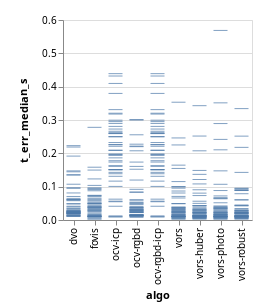
\includegraphics[width=\linewidth]{assets/img/rpe-2019-04-04.png}
	\caption{Relative pose error (rpe)}%
	\label{fig:rpe-eval}
\end{figure}

En moyenne, notre algo robuste est le meilleur. Plus d’infos sur le code d’évaluation dans le readme du dépot. Plus d’infos sur notre algo dans la section sur vors.

\section{Visual Odometry in Rust (vors)}%
\label{sec:vors}

Ce qui a démarré comme un espoir d’apporter des améliorations aux algos d’odométrie visuelle existants (en particulier DSO [github]) s’est fini en une récriture, de zéro, d’un “framework/library” d’odométrie visuelle en Rust. Les avantages techniques de Rust par rapport à C++ sont nombreux pour repartir d’une base saine mais je ne m’étends pas plus là-dessus (plus d’info dans le readme).

Le coeur d’un algo d’odométrie visuelle directe, c’est la minimisation d’une énergie de reprojection des pixels d’une image de référence à une nouvelle image. Ce problème est souvent qualifié “image alignment” par simplification dans les cas où la fonction de reprojection conserve la “topologie?” de l’image originale 2D (transformations dans le plan).

En 3D, la reprojection nécessite de connaître la profondeur d’un pixel. Le cadre le plus simple pour re-coder un algorithme de zéro, c’est donc celui du tracking caméra RGB-D (D pour depth).

Actuellement, l’algorithme implémenté dans vors est constitué des étapes suivantes :
- Générer une image multi-résolution, en teintes de gris, de l’image “keyframe”.
- Générer une image multi-résolution, en teintes de gris, de l’autre image à tracker.
- Choisir des points candidats sur le keyframe, qui vont être utilisés pour l’énergie à minimiser.
- Résoudre par un algorithme itératif (Levenberg-Marquardt) le calcul de la transformation caméra entre la keyframe et la nouvelle image :
  - Calculer le Jacobien et la Hessienne approximée (approximation de Gauss-Newton, version Levenberg-Marquardt) pour chaque résidu de l’énergie à minimiser.
  - Calculer le pas d’itération.
  - Mettre à jour la transformation caméra en compositionnel inverse
- Décider si on doit changer de keyframe.

Cette version, simple mais fonctionnelle donne d’excellents résultats sur le dataset synthétique, meilleurs que les autres algos évalués (sauf ICP). Sur le dataset réel, les résultats sont un tout petit peu en retrait comparé à DVO, fovis et OpenCV. Comme visible sur le graphique de la partie précédente, les résultats sont donc en moyenne équivalents. J’ai donc figé cette version du code, comme la version 0.1. J’en ai profité pour clarifier et documenter tout le code de cette version pour en faire une bibliothèque de l’écosystème Rust. J’y ai inclus un ensemble d’exemples d’utilisations de la lib, documentés et imagés dans le readme du dossier “examples/” du dépot.

[image] Figure représentant le processus de sélection des points candidats, qui est un des codes d’exemples.

[image] Figure représentant un exemple d’utilisation du code d’optimisation de Levenberg-Marquardt pour déterminer la transformation affine 2D entre deux images. Cet exemple sert de problème simplifié (Jacobien et Hessienne simples) pour notre problème de tracking caméra 3D. Il repose tout de même sur la même structure d’algorithme et constitue donc un excellent point d’entrée pour comprendre la version 3D caméra.

Améliorations de vors pour publications
-----

Une fois notre base vors posée. On s’est donc posé la question : “Quelles améliorations peuvent être rapidement explorées pour nous permettre d’être meilleurs que les autres algorithmes de manière consistente, y compris dans le dataset réel ?”.

Plusieurs points se sont dégagés assez rapidement, en particulier :
- Intégrer des termes photométriques dans le résidu, passer de : I\_j [ w(p) ] - I\_i [ p ]
À : a\_j * ( I\_j [ w(p) ] - b\_j )  -  a\_i * ( I\_i [ p ] - b\_i )
Ou a et b sont des termes constant dans l’image associée. Ces termes, en particulier le a permettent de prendre en compte les variations d’exposition automatiques courantes dans les séquences vidéos où l’intensité lumineuse globale de la scène varie.
- Rendre le problème de minimisation d’énergie robuste aux données aberrantes.

J’ai donc commencé en début de semaine dernière par l’amélioration avec les termes photométriques. Ça n’a pas donné ce que j’espérais. Les résultats étaient pires qu’avant. Je soupçonne que ce soit les les grands résidus (avant l’approche robuste) qui dégradent les termes photométriques plus qu’ils ne permettent d’améliorer la situation.

Je me suis donc penché en fin de semaine dernière (cf mails) sur la robustesse de la minimisation d’énergie avec deux fonctions de perte robustes :
- Huber, comme dans DSO
- Geman-McClure : x -> x\^2 / (a + x\^2)

Après rebondissements, cette fois on obtient des résultats meilleurs ! (mais pas de beaucoup)

Surtout, cette amélioration est assez sensible au choix des paramètres associés. Sachant que pour l’instant, ces paramètres sont définis globalement. J’ai été assez surpris cependant que les résultats ne soient pas meilleurs, sachant qu’ils sont environ 20\% meilleurs sur 4 des 5 datasets que j’ai testés sur mon ordinateur pendant la phase de “tuning”.

La liste des pistes d’améliorations est longue. Celle qui me semblent importantes à explorer sont les suivantes :
- Essayer une méthode statistique (déjà codée) pour construire les cartes de profondeur (semi-dense) multi-résolutions utilisées dans les itérations du problème de minimisation.
- Adapter la méthode de sélection des points candidats pour
  - 1. Améliorer la détection des points de courbures (pour l’instant on peut facilement perdre des bordures)
  - 2. Limiter le nombre de points maximum, et donc par la même occasion le rapport de densité de points entre les zones à forts et à faibles gradients. Si le rapport de densité est trop élevé, ce qui arrive assez rapidement avec beaucoup de niveaux de résolution, les points à faible gradients deviennent négligeables dans le problème de minimisation.
  - Essayer directement avec DSO aussi
- Adapter la méthode de calcul des gradients multi-résolution
  - Tester avec uniquement les gradients DSO (centrés, même résolution)
  - Tester avec des blocs 2x4 et 4x2 au lieu d’uniquement 2x2 pour ne pas “sauter” des gradients à certains niveaux de résolution.

Paramètres présents dans le code
---------------------

La multiplication du nombre de paramètres dans le code n’est pas une bonne chose. Voici donc une liste complète des paramètre réglables ayant une influence sur les performances du tracking caméra. L’objectif est de réduire ce nombre au stricte minimum.

- nb\_levels = 6 -> C’est le nombre de niveaux dans la pyramide de résolutions. En pratique, j’ai estimé (empiriquement) que 200 points à la plus faible résolution semble avoir des bons comportements. On pourrait donc déjà remplacer 6 par round( 1 + log\_4( pix / 200 ) ) pour avoir toujours environ 200 points.
- candidates\_thresh = 7 -> C’est le seuil utilisé pour la décision de prendre 2 points candidats au lieu d’un seul à la résolution supérieur lors de la sélections des candidats avec la méthode “coarse to fine”.
- max\_candidates = ? -> Ce n’est pour l’instant pas fixé, ce qui peut créer de fortes différences de densités …
- Les coefficients de Levenberg-Marquardt, (start = 0.1, multipliers = (10, 0.1) ).
- Critère d’arrêt des itérations : variation d’énergie < seuil. Ce seuil n’est pas le même suivant l’approche (robuste, …).
- Critère de changement de keyframe : optical\_flow > 1.0. J’ai essayé plusieurs valeurs pour ce critère. “Optical\_flow” est calculé comme la moyenne des déplacements des pixels entre la keyframe et l’image courante à la plus faible des résolutions de la pyramide.

Les paramètres liés aux implémentations robustes :
- Le seuil à partir duquel un résidu est abandonné (pas ajouté dans les jacobiens). Pour le moment ce seuil a donné des résultats pas trop mauvais à 50.
- Le coefficient “de coupure” correspond à l’approche robuste associée. Intuitivement, le point de bascule entre la zone convex et la zone concave de la fonction.

\subsection{Coarse to Fine Candidate Points Selection}%
\label{sub:candidates}

\subsection{Multi-Resolution Image Gradients}%
\label{sub:multires-gradients}

\subsection{Multi-Resolution Direct Image Alignment}%
\label{sub:multires-direct-image-alignment}

\subsection{Levenberg-Marquardt Optimization}%
\label{sub:lm-optimization}

\subsection{Gradients of the Reprojection Function with an Inverse Compositional Formulation}%
\label{sub:gradients-inverse-compostional}

\subsection{Robust Optimization Techniques}%
\label{sub:robust-optim}

\subsection{Photometric Term in the Residuals}%
\label{sub:photometric-residual}

\subsection{Port of VORS to WebAssembly}%
\label{sub:vors-port-wasm}

(1) how to get/capture images in a Web browser -> usage of a tar archive
(2) performances issues with realtime PNG decoding


\section{Interactive VORS on the Web}%
\label{sec:interactive-vors}


\subsection{Interactions}%
\label{sub:interactions}

We have been experimenting with different interactive modalities.
Actually, we would have liked to experiment with multiple modalities.
Here is a screenshot of the Web application Interactive vors.

\begin{figure}[h]
	\centering
	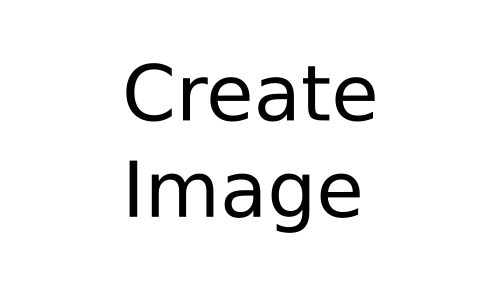
\includegraphics[width=\linewidth]{assets/img/todo.png}
	\caption{Interactive visual odometry on the Web}%
	\label{fig:interactive_vors}
\end{figure}

As you can see, the interface is split in three parts

\begin{itemize}
	\item The timeline
	\item The 3D visualization
	\item The image thumbnail of the current keyframe
\end{itemize}

The timeline enables movement along the temporal axis.
It is a one-dimentional control that is well known thanks to its pervasive use in video playing.
Visual Odometry has the advantage of dealing with video data,
contrary to structure from motion, where images are not guaranted to be in any specific order.
The timeline is thus very adapted for temporal navigation in the video.
The frames accessible from the timeline are only the keyframes of the video tracking.
Those are the frames that are used to track the following frames of the sequence.
The decision to consider a new frame as a keyframe follows a heuristic based on
the amplitude of the movement of the optical flow.
The objective is to optimize the number of keyframes in the video.
If the keyframe and the new frame are close enough,
the motion of the keyframe can be precisely estimated related to the keyframe.
So even small drifts happen during tracking, it is not additive until we change of keyframe.
Once a keyframe changes, all successive frames that will be tracked based on this keyframe
will consequently have an absolute position drift dependent of the drift of the previous keyframe.
So increasing the number of keyframes should reduce the risk of loosing completely the tracking,
but also increases the additive drift accumulated for each keyframe.

For every keyframe, we use the depth image and choose a limited amount of points
for the tracking of the following frames.
This is explained by the ``coarse to fine candidates points selection'' section.
The number of points used in each keyframe is variable but in the order of a thousand
to ten thousands points.
Those 3D points are stored in an array,
and used for a point cloud visualization with a library called ThreeJS.

The Rust ecosystem is still lacking in the domain of graphical user interfaces (GUI).
As of 2019, only a handful of libraries enable 3D graphics,
often as bindings to other C++ libraries.

%%%%%%%%%%%%%%%%%%%%%%%%%%%%%%%%%%%%%%%%%%%%%%%%%%%%%%%%%%%%%%%%%%%%%%%%%%%%%%%%
\alert{The following is an extract of the ``comptes rendus'' google doc}

\textbf{Work on 3D visualizations}
Pour une application interactive d’odométrie visuelle, il est primordial d’avoir une visualisation du nuage de points généré par les keyframes, et utilisé pour le tracking. Je me suis donc intéressé aux différentes approches de rendu avec Rust. Je conseille de lire cet article de Simon Heath (@icefoxen) intitulé “A Guide To Rust Graphics Libraries 2019”.

\textbf{Petit tour rapide des APIs de rendu.}

En dehors des programmeurs de pilotes de cartes graphiques, personne n'écrit directement du code pour GPU. À la place, on utilise des bibliothèques graphiques telles que OpenGL. Aujourd'hui, les 4 principales APIs graphiques utilisables sont OpenGL, DirectX, Vulkan et Metal.

OpenGL est un standard ouvert, développé par le groupe Khronos, qui a vu le jour en 1992. Des pilotes existent pour presque tous les systèmes, linux, windows, osx, etc. Son principal problème est son âge. C'est une API assez haut niveau qui n'a pas évolué favorablement en comparaison des architectures des GPUs.

DirectX (DX) est un peu l'équivalent d'OpenGL à la sauce Microsoft, disponible uniquement pour Windows et XBox. Jusque DirectX 11, les API sont très haut niveau, comme OpenGL. DirectX 12 la dernière version fait parti d'un renouveau de pilotes plus bas niveaux, tout comme Vulkan et Metal, qui tirent beaucoup mieux parti des architectures actuelles des cartes graphiques.

Vulkan est à OpenGL ce que DX12 est à DX11, une API bien plus bas niveau mais offrant des bien meilleures performances. J'ai le sentiment que sur des appareils de faibles puissance, tels que des smartphones, la différence se fera bien ressentir et il sera courant d'avoir des perf x2, x3 ou plus suivant les cas.

Metal c'est le DX12 d'Apple. Une API bas niveau uniquement accessible sur des machines Apple.

\textbf{Et Rust dans tout ça ?}

En Rust, il y a des wrappers pour chacune des APIs graphiques, souvent le nom de l'API suffixé "-rs" (pour rust). Ces bibliothèques ont souvent une API "unsafe", ce qui signifie en Rust qu'elles n'ont pas toutes les garanties que peut apporter le langage en terme sûreté mémoire. La bibliothèque probablement la plus important de l'écosystème graphique de Rust s'appelle "gfx", aujourd'hui renommée "gfx-hal" (pour hardware abstraction layer). C'est une API bas niveau, à 97\% similaire à Vulkan mais qui est multi-plateforme ! Elle peut compiler vers Vulkan, DX12, ou Metal suivant l'environnement (et un support réduit d'OpenGL). Il existe aussi une bibliothèque très active du nom de "rendy" qui se veut être un toolkit pour gfx-hal et réduit la quantité de boilerplate nécessaire pour des APIs autant bas niveau.

\textbf{Et le Web dans tout ça ?}

Et bien justement, on est là aussi au bord d’un renouveau complet. Tout comme WebGL qui a apporté une version simplifié et sécurisée d'OpenGL sur le Web en 2011, le W3C, en collaboration avec Apple, Mozilla, Microsoft et Google, est en train de standardiser une API dédiée au Web, du nom de WebGPU. WebGPU devrait exposer pour JavaScript et WebAssembly une API graphique et de calcul (comme Cuda / OpenCL) efficace pour tout appareil ayant des pilotes natifs pour Vulkan / DX12 / Metal.

L'implémentation de WebGPU en Rust, qui s'appelle "wgpu", a démarré vers Septembre 2018. La où ca devient encore plus intéressant, c'est qu'elle est basée sur gfx-hal pour le rendu. Utiliser wgpu permet donc en théorie d'avoir un code efficace, un peu plus haut niveau que Vulkan, compilable vers toutes les plateformes natives et le Web ! En pratique malheureusement, au jour d'aujourd'hui (aout 2019), seul Chrome canary sur OSX supporte WebGPU. On ne peut donc pas (encore) s'en servir pour des applis Web. Mais vu la motivation des différents partis, ça devrait arriver vite !

\textbf{C’est beau mais en pratique on fait quoi nous ?}

De l'OpenGL / WebGL mon capitaine ! J'ai donc cherché dans l'écosystème Rust, et je suis tombé sur Kiss3D, par le même créateur que la bibliothèque d'algèbre linéaire que j'utilise. Kiss3D promet une API simple et compatible avec WebAssembly. Après quelques essais ratés, les premières visualisations correctes sont encourageantes ! Je raconte mes pérégrinations dans ce post du forum rust pour de plus amples détails.


https://youtu.be/hCzT47eeges


Mais (comme toujours il y a un mais ...) malheureusement la compilation vers wasm fait drastiquement chuter les performances sur mon ordi portable. On passe d'environ 60 fps en natif à environ 10 fps en web, ce qui n'est clairement pas utilisable. Il y a également une deuxième chose qui m'a chagriné. Kiss3D est basé sur "stdweb" pour sa compilation vers wasm. Or "stdweb" est une approche alternative à l'approche standardisée pour wasm en Rust, qui s'appelle wasm-bindgen, et les deux ne sont pas facilement compatibles. Il est donc difficile de faire cohabiter le code de tracking, utilisant wasm-bingen, et le code de visualisation, basé sur stdweb.

\textbf{Finalement on fait quoi du coup ?}

L'approche qui me donne le meilleur compromis de performances et de flexibilité, c'est de mixer les calculs faits en Rust + wasm (en utilisant wasm-bindgen), avec le rendu fait en JavaScript avec Three. Three c'est probablement la bibliothèque de 3D la plus mature pour le Web, avec une API simple en JavaScript. C’est celle que Thomas utilise pour ses rendus. En faisant tous mes calculs avec Rust, je peux partager avec Three un pointeur vers la position dans la mémoire wasm du résultat des calculs. Le seul léger inconvénient, c'est que toute donnée nécessaire pour le rendu Three, doit avoir un attribut permanent associé dans le code Rust. C'est un moindre mal, et en utilisant correctement l'API Three, j'obtiens 25 à 30 fps pour un million de points avec mon ordi portable. Axel a un solide 60 fps sur son ordi.

Voici la démo, et le code source pour un simple exemple générant un cube rempli d'un million de points aléatoires. Je suis curieux de savoir à quel framerate cet exemple tourne dans différents types d'appareils mobiles. Avec mon android bas de gamme, j'obtiens 4 fps sous chrome, et 3 fps sous firefox.

La démo la plus intéressante, c'est celle de l'appli de tracking vors ! Elle est disponible ici, code source par là. ATTENTION, pour la faire tourner, il faut 1.6 Go de ram disponible avec le dataset ICL NUIM. Pour démarrer la démo, il faut lui donner une archive tar contenant tout le dataset à tester. Il y a une archive (700 Mo) toute prête, téléchargeable jusqu'au 29 aout par ici. Ci-dessous une capture d’écran de l’appli qui tourne sur mon ordi portable.

\alert{End of the google doc extract.}
%%%%%%%%%%%%%%%%%%%%%%%%%%%%%%%%%%%%%%%%%%%%%%%%%%%%%%%%%%%%%%%%%%%%%%%%%%%%%%%%

As we explain in the extract above,
we ended using ThreeJS for the 3D visualization.
Upon navigation in the timeline, there are two other different modifications of the visualization.
First the 3D points corresponding to the current keyframe are displayed in another color (red),
and the camera point along the camera trajectory is updated.
This makes following the camera trajectory and identifying the associated geometry trivial.
And second, the thumbnail of the current keyframe is updated.
As a consequence, looking at the thumbnail area while moving along the timeline
reminds temporal navigation in traditional 2D videos.
It also facilitates the association of the 3D geometry with the actual 2D frame
from the original video sequence.
In sum the combination of a keyframe timeline with associated thumbnail
and 3D geometry bridges the traditionally difficult gap between 2D and 3D user interfaces.

We just have introduced the first interactive modality, the keyframe timeline navigation.
In order to introduce the other two, we need to describe first
a problem we are facing with our visual odometry algorithm.
The video sequences used for the benchmark of the different visual odometry algorithms
have different difficulty levels of tracking.
The synthetic sequence from the ICL NUIM dataset
have the particularity of providing low textured but crisp images with perfect alignment
between the color images and depth map.
Those conditions enable high precision tracking, except for some short sections
almost not textured at all, where tracking is lost and drifts.
When running interactive vors on this dataset,
we observe two of those distinctive drifts, resulting in multiple
disjoint and unaligned pieces of the global 3D model of the associated room.

\begin{figure}[h]
	\centering
	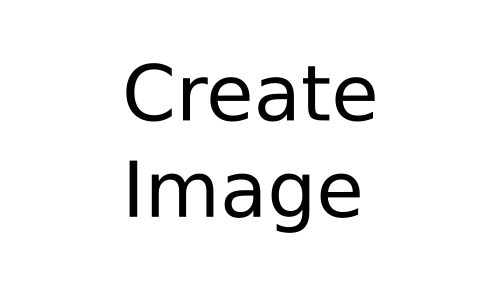
\includegraphics[width=\linewidth]{assets/img/todo.png}
	\caption{Misaligned 3D model due to drifts in the tracking.}%
	\label{fig:drift_icl_nuim}
\end{figure}

If we set for example the objective to obtain a globally coherent 3D model of the room,
there are plenty of approaches heading in that direction.
Here are two of those.

\begin{itemize}
	\item Identify in the timeline each section with a coherent 3D model associated.
		Export a model of each temporally coherent section.
		Join all parts of the model with an approch such as ICP (Iterative Closest Point).
	\item Identify two keyframes in the timeline with a visual overlapping
		but no 3D geometry overlapping due to a drift between those images.
		Re-align those two images.
		Adapt the tracking of the rest of the sequence to take into account this adjustment.
\end{itemize}

We decided to take the second approach for this experiment.
The second option here is very similar to what we usually call SLAM.
SLAM consists in adding loop closure and pose graph optimization techniques
to visual odometry to bring global map consistency.
In traditional SLAM algorithms, points of interests are retrieved for all keyframes.
Their descriptors are classified with techniques like ``bag of words''.
Then typical indexing and search techniques are applied to identify similar keyframes.
In our case, the identification is performed by a human interaction.
Once two keyframes are matched, the next step consists in computing
the camera motion between those.
Usually, one would match all keypoints in the pair of images
and use a robust version of the 8-point algorithm if there is no depth info,
or a robust PNP algorithm if depth info is know.
Logically, we thus tried to perform keypoints detection and matching for the pair of keyframes.
There exist many keypoint descriptors for this task.
Some well known are ORB, SIFT, FAST, A-KAZE.
The A-KAZE features were already implemented in Rust (https://github.com/indianajohn/akaze-rust)
so we tried to use them for the matching.
Unfortunately, due to the low textured images of the synthetic dataset,
the number of matches for selected pairs of keyframes were in the order of 20,
not enough to compute reliable camera motion.
This is the origin of the next two interactive modalities explored.

Once a pair of keyframes is identified by a user,
thumbnails of those two frames are displayed next to each other.
The reference keyframe thumbnail also displays in red the points used for the tracking,
i.e. points which also provide depth information.
We consciously restrict the number of points with depth information to candidates
points used in the tracking, instead of all points with depth information from the sensor,
for two reasons.
(1) Those points are the only points supposed to be known if we extend our work to RGB visual odometry,
(2) less red points means less visual clutter for the user.
In those two thumbnails, the user is asked to identify three pairs of points
by clicking inside the two images.
In the reference image, the points chosen should be restricted to those in red.
From the three pairs of points, we can compute 0 to 4 potential camera positions
based on the P3P algorithm.
Since there was no currently available Rust P3P implementation,
and it was not too complicated to implement, we ported M. Persson ``Lambda Twist''
P3P algorithm. It is available at https://github.com/rust-photogrammetry/p3p.
Those potential camera positions are used to backproject the points with known depth
(red points in the thumbnail) into the 3D environment.
Every potential camera pose is associated with 3D points of a unique color
as depicted in Figure~\ref{fig:p3p}.

\begin{figure}[h]
	\centering
	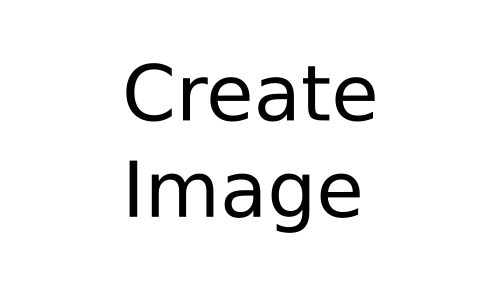
\includegraphics[width=\linewidth]{assets/img/todo.png}
	\caption{P3P camera pose candidates.}%
	\label{fig:p3p}
\end{figure}

As also visible in Figure~\ref{fig:p3p}, a probability is associated with every potential pose.
Those probabilities are estimated by a measure of photometric reprojection error.
Indeed, for each potential camera pose, it is possible to project the 3D points
of the reference keyframe into the other frame.
For this estimatation we compute the reprojection error at low resolution images
which are less sensible to small errors in the reprojection.
In the end, the probability scores are simply set proportional to the inverse of the reprojection errors.
Such scores are intended to be a hint for the user,
helping them to select the correct pose initialization in the interface.
With this combination of colored 3D visualization and selectable options,
we avoid the complex task of directly interacting in the 3D world.
In the end, the chosen pose is set as initialization to the tracking algorithm.
The tracking is then restarted from this second keyframe.
It should provide a globally consistent 3D model until the next drift in the sequence.

\subsection{Drawbacks of the approach}%
\label{sub:drawbacks}

In traditional SLAM, the loop closure and pose estimation would add
an edge in the global pose graph of the sequence.
Then a pose graph optimization algorithm would be run to improve the global
consistency of the pose graph.
In our simplified case however, we do not build this pose graph,
but simply ensure the coherence of the sequence after the second keyframe
with regard to the reference keyframe.
It means that all frames in between the pair of keyframes is not adjusted.
In particular, there will still be drifted frames in this section of the sequence.

\subsection{Code architecture of interactive VORS}%
\label{sub:code-interactive-vors}

The code of this project is available at https://github.com/mpizenberg/interactive-vors.
As of version 1.0.0, it is composed of three main parts.
Those are clearly reflected by the language percentage usage in GitHub Web page interface,
38\% JavaScript, 35\% Elm and 26\% Rust.

The Elm application manages the Web user interface and communicates
with the JavaScript part to handle the 3D drawing and visual odometry.

The 3D rendering is handled by a JavaScript library called ThreeJS, based on WebGL.
A keyframe may contain 1 to 10 thousand points with depth information.
In a typical tracking situation, there might be one keyframe for rougly 5 to 20 frames.
The ICL-NUIM sequence for example, is composed of 1508 frames,
and results in 225 keyframes and 550000 points.
Being able to display point clouds with a number of points in the order of the million
with WebGL is still a non trivial task for today mid-end hardware.
In order to mitigate 3D drawing performance bottlenecks,
all the 3D visualizations in the application are based on a unique preallocated
geometry buffer sized for a million point.
While it is a reasonable solution for our proof of concept use case,
this is an important detail if we are to consider more memory efficient solutions.
We will also note, that with the advent of the new standard WebGPU,
better performances and compatibility with WebAssembly are to expect in the near future.

The visual odometry algorithm is of course a WebAssembly module,
compiled from a small Rust interface module,
reusing our Rust visual odometry algorithm (vors).
Our JavaScript code base is communicating with this Wasm module
thanks to the intermediate JavaScript binding code generated by wasm-bindgen and wasm-pack.
Before diving into the details of porting vors to WebAssembly,
we will provide few quantitative measures of the improvements that our interactive
approach enabled.

\subsection{Quantitative improvements of the 3D model and trajectory}%
\label{sub:quantitative-improvements}

(1) absolute trajectory error
(2) absolute point cloud error
